% =====================================================================
%  G1 - Homomorphic tally time vs voter count
%  --------------------------------------------------------------------
%  Backs the claim: O(n) linear tally with ~6.1 microsecond per vote
%  Source: chapter4.tex Table 4 (tab:tally-scale)
% =====================================================================
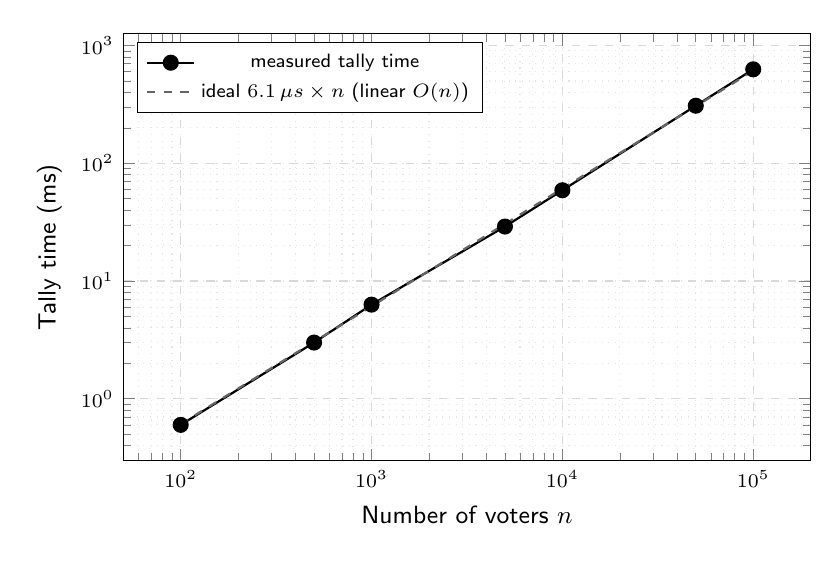
\begin{tikzpicture}
\begin{axis}[
    width=0.85\textwidth,
    height=7cm,
    xlabel={Number of voters $n$},
    ylabel={Tally time (ms)},
    xmode=log,
    ymode=log,
    log basis x=10,
    log basis y=10,
    grid=both,
    grid style={dashed, gray!30},
    minor grid style={dotted, gray!20},
    legend style={at={(0.02,0.98)}, anchor=north west,
                  font=\sffamily\scriptsize, draw=black},
    label style={font=\sffamily\small},
    tick label style={font=\sffamily\scriptsize},
    every axis plot/.append style={thick},
]
% Measured points from Table tab:tally-scale
\addplot+[mark=*, mark size=2.5pt, color=black, mark options={fill=black}] coordinates {
    (100,    0.6)
    (500,    3.0)
    (1000,   6.3)
    (5000,  29.0)
    (10000, 59.0)
    (50000, 308.0)
    (100000, 628.0)
};
\addlegendentry{measured tally time}
% Reference line: ideal linear at 6.1 microseconds per vote
\addplot[domain=100:100000, samples=100, dashed, thick, color=black!60]
   {6.1e-3 * x};
\addlegendentry{ideal $6.1\,\mu s \times n$ (linear $O(n)$)}
\end{axis}
\end{tikzpicture}
